\documentclass[a4paper,11pt,titlepage]{article}


\usepackage[italian]{babel}

\usepackage{graphics}

\usepackage[dvips]{graphicx}

\usepackage[latin1]{inputenc}

\usepackage{verbatim}

\usepackage{makeidx}

\usepackage{fancyhdr}

\usepackage{color}

\usepackage{syntonly}

\usepackage{amsfonts}

\usepackage{amsmath}

\usepackage{amssymb}


% stile di pagina

\pagestyle{fancy}


% autore

\author{Dario Di Minno \and Claudio Tortorelli}


\makeindex



\begin{document}

\hyphenation{Di-se-gna-to-re Li-sta-U-ten-ti-fo-rum e-re-di-ta-no}

\title{Relazione per il corso di \\ Linguaggi di Programmazione: \\ Metodologie di Programmazione}

\thispagestyle{empty}

%\renewcommand{\chaptermark}[1]{\markboth{#1}{}}

\renewcommand{\sectionmark}[1]{\markright{\thesection\ #1}}

\fancyhf{} \fancyhead[LE,RO]{\bfseries\thepage}

\fancyhead[LO]{\bfseries\rightmark}

\fancyhead[RE]{\bfseries\leftmark}

\renewcommand{\headrulewidth}{0.5pt}

\addtolength{\headheight}{0.5pt}

\fancypagestyle{plain}


\newcommand{\vect}[1]{\boldsymbol{#1}}



\maketitle 


\newpage


\tableofcontents %\listoffigures \listoftables


%************************************************************************


%************************************************************************

\section{Introduzione}

Lo sviluppo di un'applicazione tipicamente prevede i seguenti passi:
\begin{itemize}
\item Analisi del problema
\item Progettazione
\item Implementazione
\end{itemize}

L'analisi del problema fornisce come risultato delle specifiche precise e non ambigue sulle quali basare la progettazione.
Seguendo il paradigma della programmazione orientata agli oggetti, durante la progettazione 
vengono definite le \emph{classi} e le relazioni che intercorrono tra di loro.
Tale sistema viene rappresentato mediante un diagramma \emph{UML} e implementato in un linguaggio orientato agli oggetti. 

Partendo dal problema di realizzare un sistema di tutoraggio per studenti universitari, abbiamo affrontato i passi sopra descritti fino arrivare a un'effettiva implementazione.

\subsection{Descrizione del problema}
\label{sec:DescrizioneDelProblema}

Un \emph{servizio di tutoraggio per studenti universitari} � un sistema tramite il quale gli \emph{studenti} possono usufruire dell'assistenza di un gruppo di \emph{tutor}.

Ogni studente interessato pu� iscriversi facendone richiesta a un \mbox{\emph{amministratore}}.

I servizi che sono forniti agli studenti possono essere diversi, come:
\begin{itemize}
	\item un \emph{forum} formato da pi� \emph{gruppi di discussione}, uno per ogni materia.
	\item una bacheca
	\item posta elettronica
	\item una collezione di domande frequentemente poste
	\item e altro...
\end{itemize}

Nel nostro progetto abbiamo sviluppato il forum, in quanto parte fondamentale del sistema.


\section{Analisi}
\label{sec:Analisi}


\subsection{Casi d'uso}
\label{sec:CasiDUso}
Per scoprire i requisiti del sistema, abbiamo evidenziato le interazioni fra utente e sistema mediante il grafico dei \emph{casi d'uso}:
\\
%\begin{figure}[!h]
%      \centering
      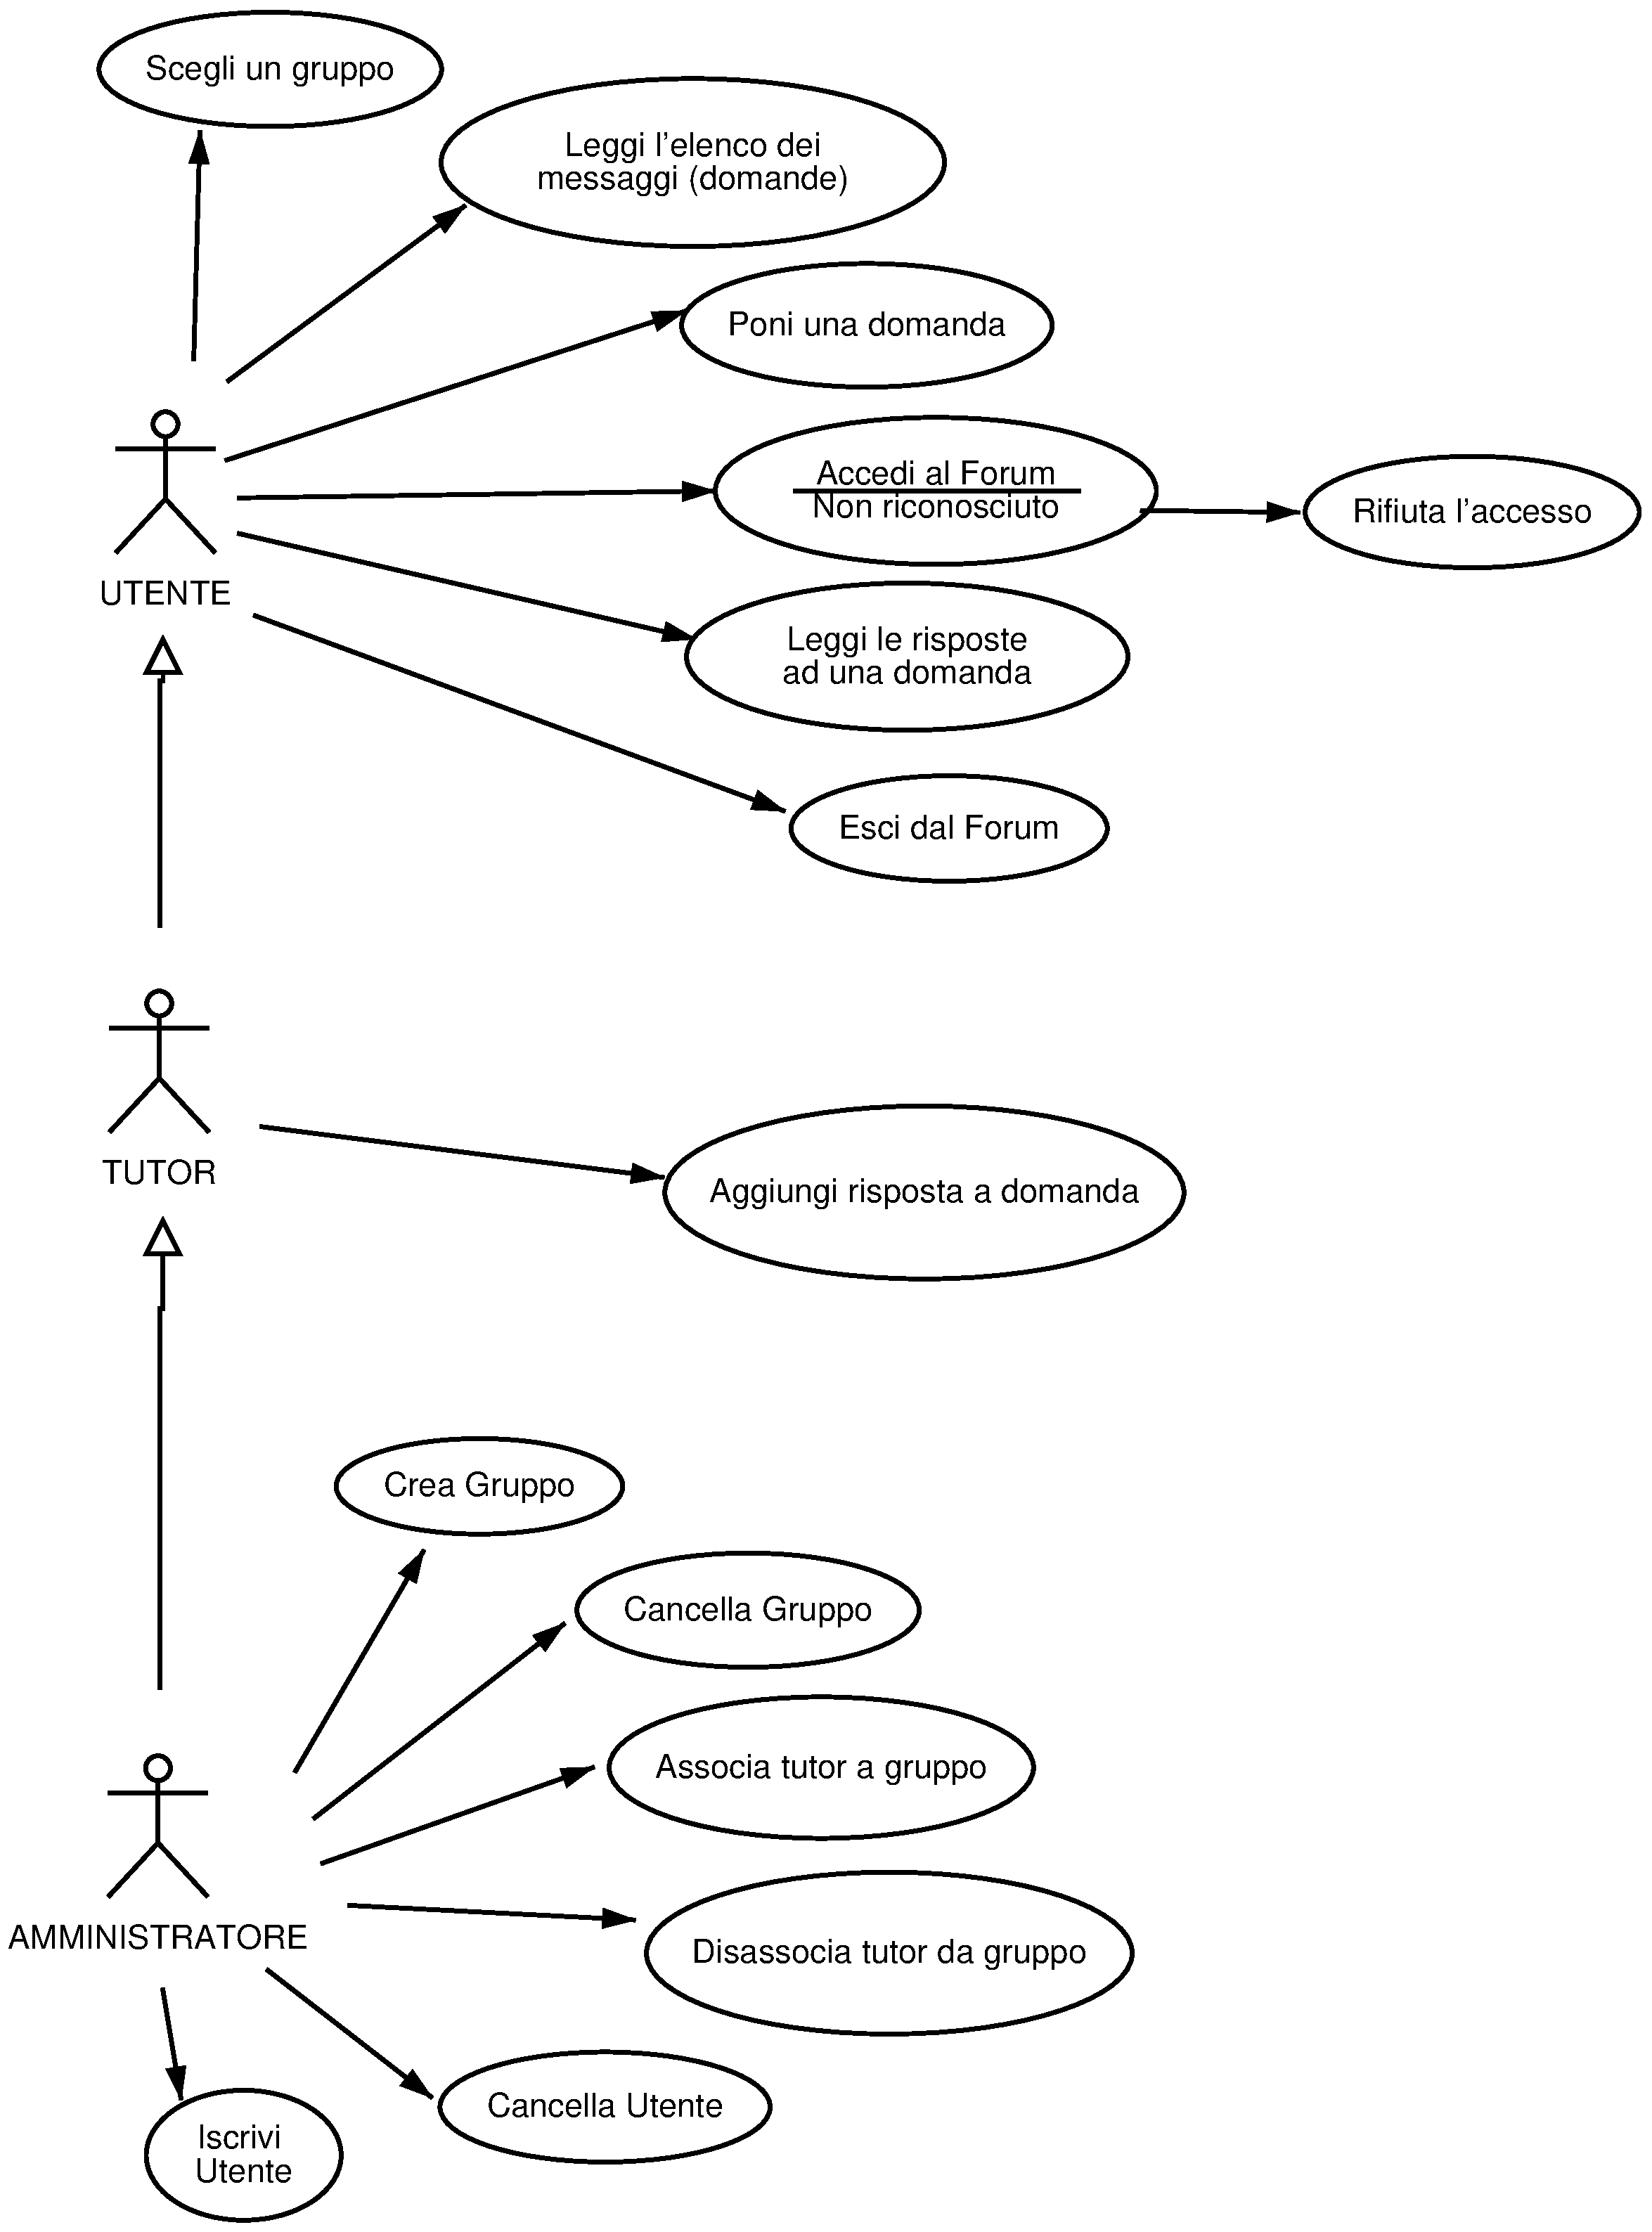
\includegraphics[angle = 0, width=\textwidth]{casiduso.eps}
%      \caption{Casi d'uso dell'applicazione}
%\end{figure}


\subsection{Specifiche dell'applicazione}
\label{sec:SpecificheDellApplicazione}

Dalla nostra analisi, sono derivate le seguenti specifiche:

Esistono tre tipi di utenti: Utente, Tutor, Amministratore.
Ogni utente � descritto dalle sue informazioni personali, pi� una login e una password per essere riconosciuto dal sistema.
Una volta entrato nel sistema, un utente semplice pu� accedere al forum, leggere le domande poste nei gruppi di discussione e porre nuove domande. 
I tutor sono degli utenti con la possibilit� di rispondere alle domande poste nei gruppi ai quali sono associati.
Gli amministratori sono tutor con la facolt� di:
\begin{itemize}
 \item aggiungere o cancellare gruppi di discussione del forum
 \item gestire le associazioni fra tutor e gruppi
 \item gestire le iscrizioni degli utenti
\end{itemize}

Se il sistema non possiede utenti, al suo avvio crea un amministratore con login "`root"' e password "`root"'. Questo primo utente creer� poi gli altri.

\section{Progettazione}
\label{sec:Progettazione}

\subsection{Uso di pattern}
\label{sec:UsoDiPattern}
L'utilizzo di un pattern influenza significativamente la progettazione di un sistema, o perlomeno di una sua parte. Abbiamo fatto uso del pattern Command, che ci ha suggerito le linee guida per la realizzazione del men�, che � composto da voci di men� che, se selezionate, fanno partire l'esecuzione di uno o pi� comandi.

L'utilizzo di questo pattern quindi ci ha portato a definire le classi Men�, MenuItem (le voci del men�) e Command.
I comandi sono realizzati come classi che hanno la responsabilit� dell'esecuzione del comando che implementano. 
Il men� viene istanziato in forme diverse a seconda del tipo di utente che accede al sistema, abilitando o meno alcune operazioni.

\subsection{Descrizione del sistema e interazioni fra le classi}
\label{sec:DescrizioneDelSistemaEInterazioniFraLeClassi}
La classe \textbf{Sistema} ha un ruolo fondamentale nell'applicazione, in quanto crea gli oggetti che sono alla base del suo funzionamento.
In particolare, questi oggetti sono:
\begin{itemize}
 \item Forum
 \item ListaUtentiForum
 \item Disegnatore
 \item Menu
\end{itemize}

Inoltre il sistema dopo aver autorizzato un utente registrato a utilizzare il forum, delega agli oggetti che ha creato il recupero delle informazioni memorizzate in precedenza sui file.

Il \textbf{Forum} contiene i riferimenti ai gruppi di discussione e fornisce agli oggetti di classe Command l'accesso ai messaggi memorizzati. Tutta la gestione dei gruppi di discussione passa attraverso questa classe.

Un \textbf{GruppoDiscussione} � formato da un insieme di messaggi, strutturato come una sequenza di domande seguite da eventuali risposte. Le domande e le risposte sono tutte istanze della classe \textbf{Messaggio}. E' compito di GruppoDiscussione mantenere su file i messaggi in modo ordinato.

\textbf{ListaUtentiForum} ha i riferimenti agli utenti registrati nel sistema e dunque ha accesso a tutti i loro dati, permettendo il loro utilizzo alle classi che ne fanno richiesta. Questa classe si preoccupa anche di garantire la persistenza dei dati di cui � responsabile.

L'utente semplice � rappresentato dalla classe \textbf{Utente}. Da questa ereditano le classi \textbf{Tutor} e \textbf{Amministratore}, che hanno in pi� dei riferimenti a un insieme di gruppi per i quali hanno diritto a rispondere.
Le operazioni di responsabilit� dell'amministratore vengono rese disponibili dal Menu che viene a lui istanziato.

Alla classe \textbf{Disegnatore} vengono indirizzate le richieste di visualizzazione dell'output in modo da dare un aspetto omogeneo all'interfaccia utente.

La classe \textbf{Menu} possiede i riferimenti ai MenuItem, ovvero le voci di menu che possono presentarsi agli utenti. I MenuItem vengono istanziati dal costruttore di questa classe a seconda dell'utente che sta utilizzando il sistema. I \textbf{MenuItem} a loro volta hanno i riferimenti a un insieme di \textbf{Command} che implementano i comandi associati alle voci di menu disponibili. Selezionare un MenuItem equivale quindi a eseguire in maniera ordinata le Command a cui fa riferimento. Tutti i comandi sono implementati nel metodo \emph{execute()} di classi derivate da Command. Queste ultime, per eseguire i propri compiti, dispongono dei riferimenti alle classi principali del sistema (Forum, ListaUtentiForum, Disegnatore).

\subsection{Diagramma UML}
\label{sec:DiagrammaUML}
Il diagramma UML risultante dalla progettazione e dalle sue successive revisioni � il seguente:
\begin{figure}[!ht]
      \centering
      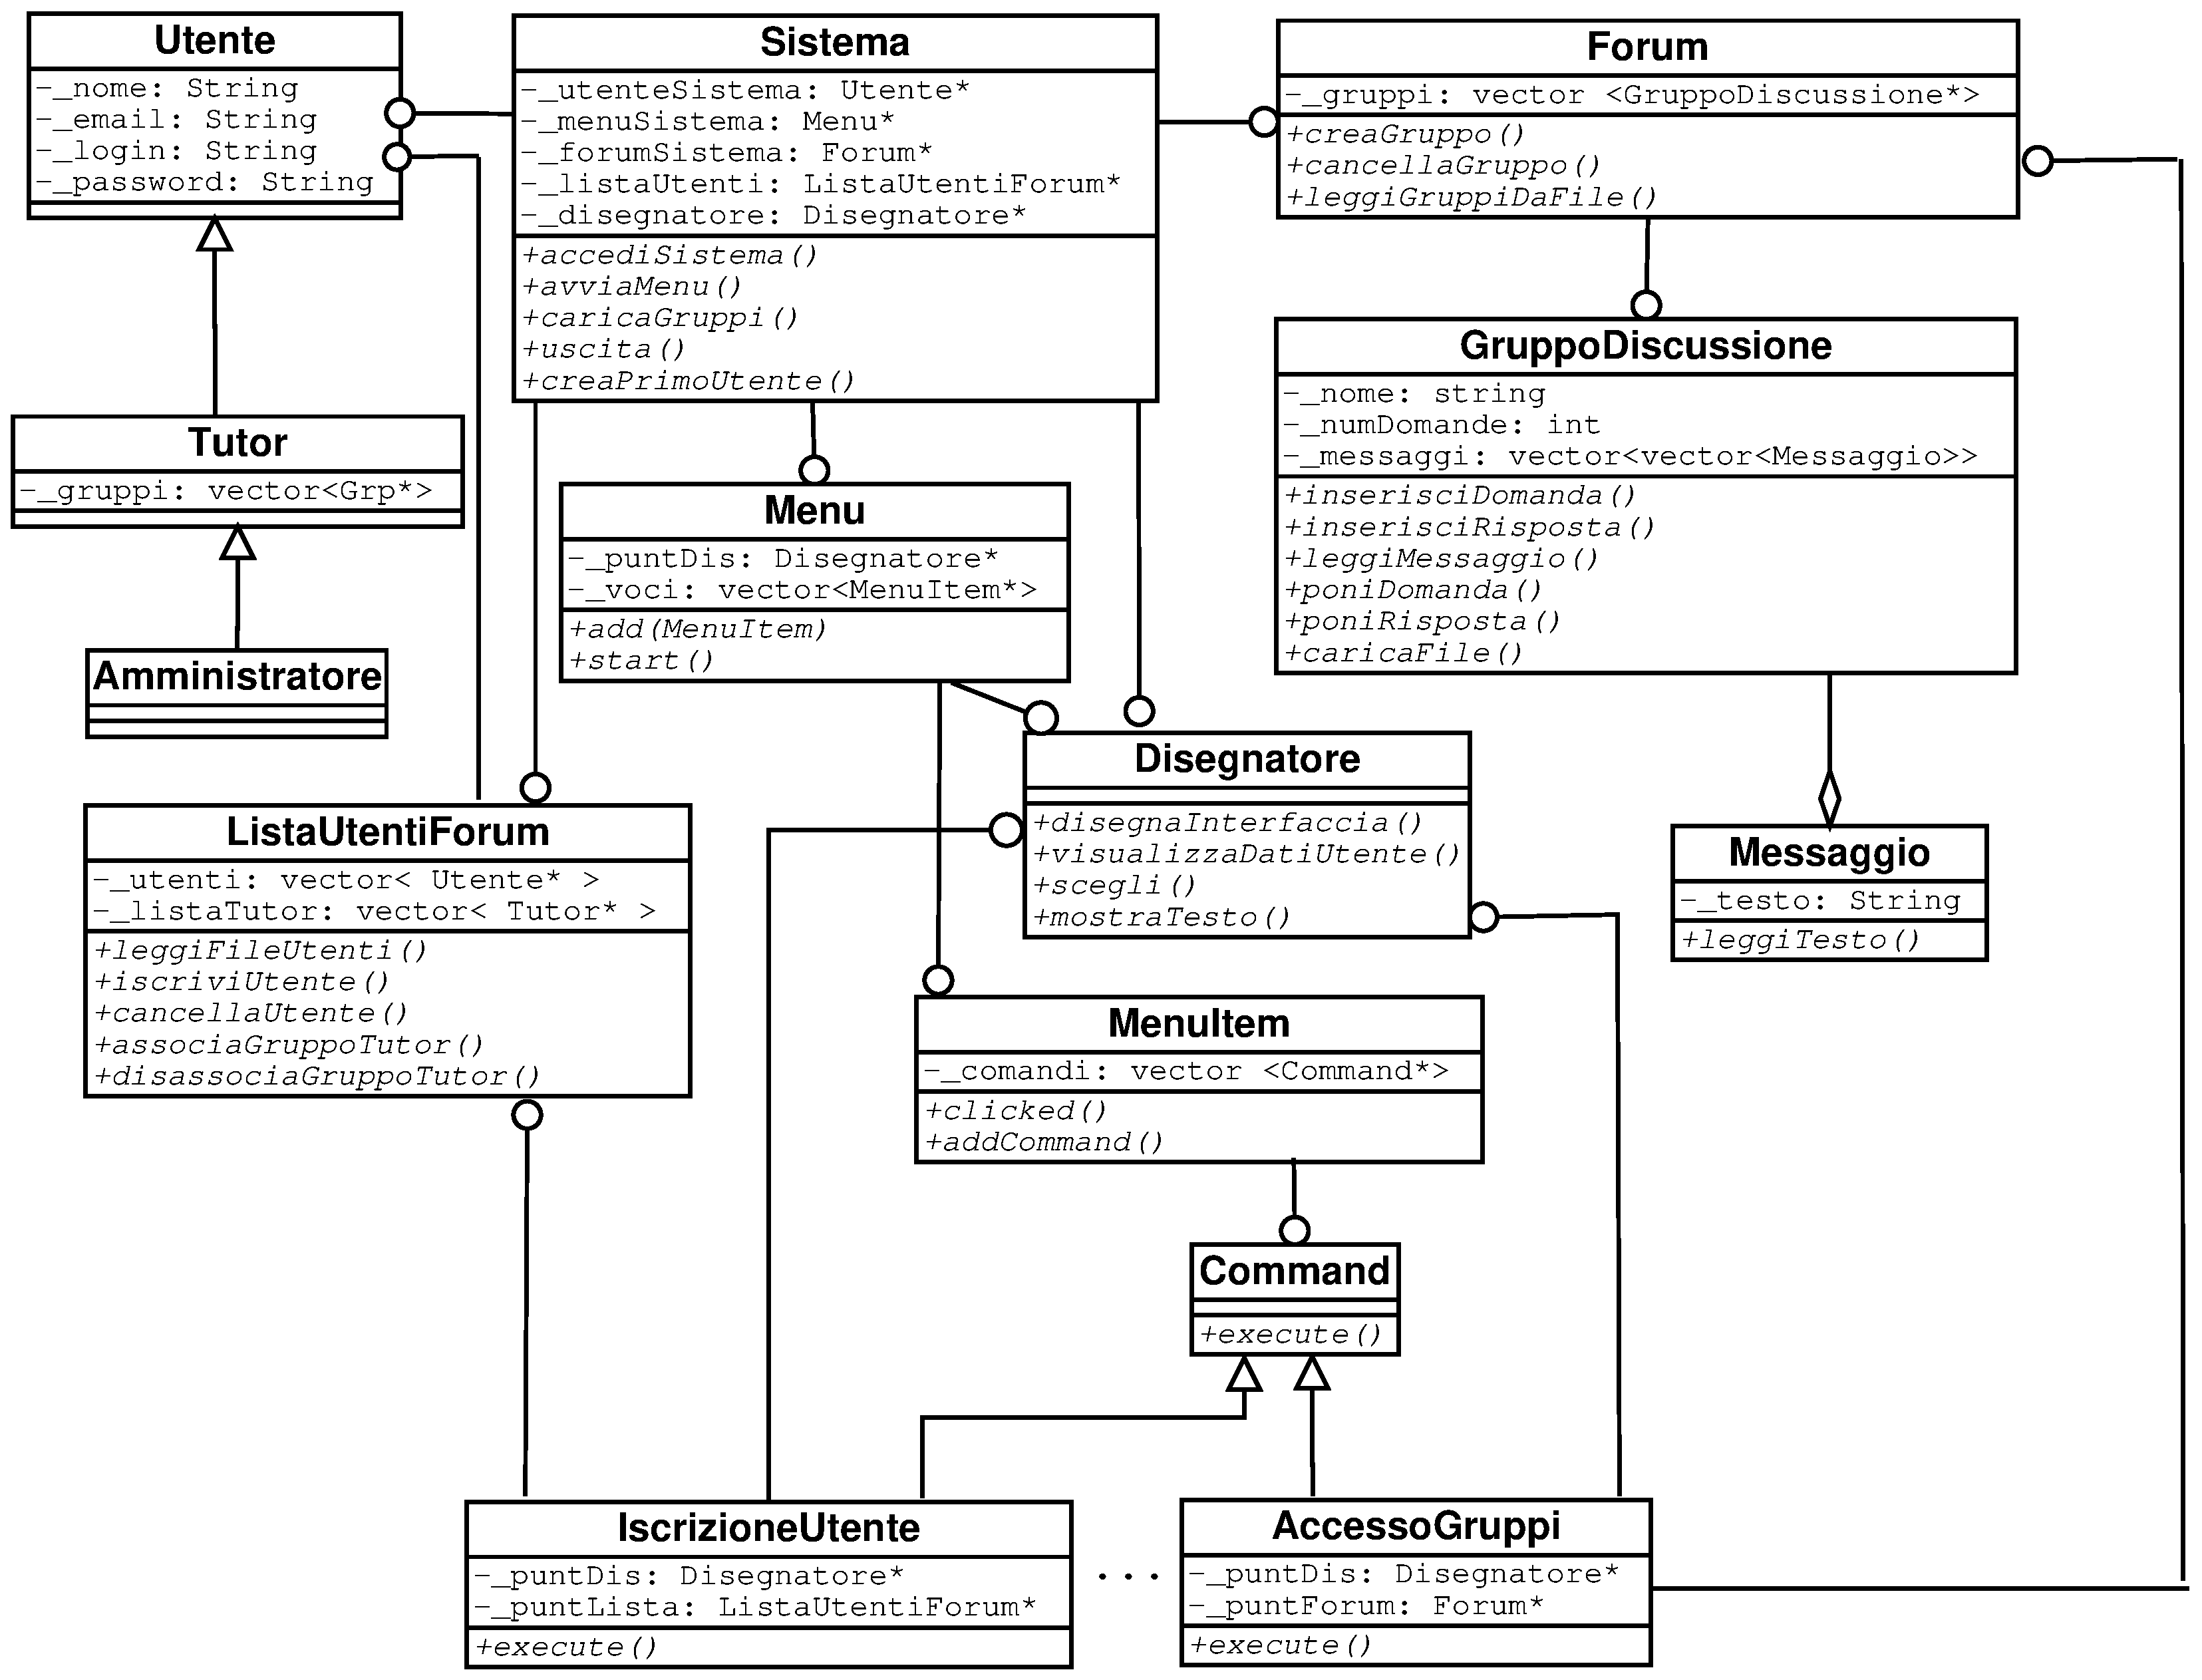
\includegraphics[angle = 90, width=\textwidth, height = \textheight]{UML.eps}
      %\caption{Diagramma delle classi}
\end{figure}



\section{Implementazione}
\label{sec:Implementazione}

\subsection{Scelte implementative}
\label{sec:ScelteImplementative}

\paragraph{Compilatore utilizzato}
\label{sec:CompilatoreUtilizzato}
Il linguaggio di programmazione da noi usato per scrivere il codice del progetto � il C++, in particolare il compilatore \emph{mingw}, ovvero il porting su sistema operativo \emph{Windows} e piattaforma Intel x86 del famoso \emph{gcc} della GNU.
In particolare ci siamo avvalsi dell'ambiente di sviluppo gratuito DEV-C++ (www.bloodshed.net/dev), versione 4.9.6.0.

\paragraph{Librerie utilizzate}
\label{sec:LibrerieUtilizzate}
Abbiamo fatto uso di librerie ANSI-C++ per la gestione di vector, stringhe, stream, date, e della libreria conio per la gestione dell'output su schermo.

%%%%%%%%%%%%%%%%%%%%%%%%%%%%%%%%%%%%%%%%%%%%%%%%%
\subsection{Documentazione delle classi}

Abbiamo suddiviso le classi nelle seguenti categorie: Command, Menu, MenuItem, Utenti, Forum, Sistema, Disegnatore, ListaUtentiForum. Segue la loro descrizione.


\textbf{Command}

%------------ACCESSO GRUPPI-----------------------*
\subsubsection{AccessoGruppi}
	\paragraph{ File:\\}			
		AccessoGruppi.h, AccessoGruppi.cpp		
		
	\paragraph{ Descrizione\\} 
	Questa classe eredita da Command e serve a visualizzare e scegliere il gruppo al quale accedere tra l'elenco dei gruppi di discussione presenti nel sistema. 
	
	\paragraph{ Costruttore} 	
	\begin{itemize}
	\item \texttt{AccessoGruppi(Forum* f, Disegnatore* d, int* sceltaGruppo)}
	\end{itemize}	
	Il costruttore di questa command richiede in input il riferimento al Forum e al Disegnatore correnti, oltre al riferimento ad un intero che � il valore di scambio tra le varie command di questo MenuItem. Nel caso della AccessoGruppi questo intero assume significato di "`sceltaGruppo"'.
			
	\paragraph{ Metodi} 
	\begin{itemize}
	\item	\texttt{virtual void execute()} 
	\end{itemize}
	Esegue il comando rappresentato.
		
%------------ASSOCIA GRUPPI-----------------------*
\subsubsection{AssociaGruppi}
	\paragraph{ File\\}			
	  AssociaGruppi.h, AssociaGruppi.cpp
		
	\paragraph{ Descrizione\\} 
	Questa classe eredita da Command e serve ad associare un particolare gruppo ad un Tutor. Questa operazione permette poi al Tutor di poter rispondere a domande di quel gruppo.
	
	\paragraph{ Costruttore} 
	\begin{itemize}
	\item	\texttt{AssociaGruppi(Forum* f, Disegnatore* d, ListaUtentiForum* l, int* numeroTutor)}
	\end{itemize}
	Il costruttore di questa command richiede in input il riferimento al Forum, al Disegnatore e alla ListaUtentiForum correnti. Inoltre vuole il riferimento ad un intero che � il valore di scambio tra le varie command di questo MenuItem. Nel caso della AssociaGruppi questo intero assume significato di "`numeroTutor"', cio� l'indice del particolare tutor nella lista dei tutor.
			
	\paragraph{ Metodi} 
	\begin{itemize}
	\item	\texttt{virtual void execute()} 
	\end{itemize}
	Esegue il comando rappresentato.

%------------CANCELLA GRUPPO-----------------------*
\subsubsection{CancellaGruppo}
	\paragraph{ File\\}			
	 CancellaGruppo.h, CancellaGruppo.cpp
		
	\paragraph{ Descrizione\\} 
	Questa classe eredita da Command e serve ad eliminare un particolare gruppo dal sistema. 
	
	\paragraph{ Costruttore} 
	\begin{itemize}
	\item	\texttt{CancellaGruppo(Forum* f, Disegnatore* d, int*	 numGruppo)}
	\end{itemize}
	Il costruttore di questa command richiede in input il riferimento al Forum e al Disegnatore correnti. Inoltre vuole il riferimento ad un intero che � il valore di scambio tra le varie command del MenuItem di cui CancellaGruppo fa parte. Nel caso della CancellaGruppi questo intero assume significato di "`numGruppo"', cio� l'indice del particolare gruppo di discussione da eliminare.
			
	\paragraph{ Metodi} 
	\begin{itemize}
	\item	\texttt{virtual void execute()} 
	\end{itemize}
	Esegue il comando rappresentato.


%------------CANCELLA UTENTE-----------------------*
\subsubsection{CancellaUtente}
	\paragraph{ File\\}			
	 CancellaUtente.h, CancellaUtente.cpp
		
	\paragraph{ Descrizione\\} 
	Questa classe eredita da Command e serve ad eliminare un particolare utente dal sistema, eccetto lo stesso utente che ne fa richiesta. 
	
	\paragraph{ Costruttore} 
	\begin{itemize}
	\item	\texttt{CancellaUtente(Disegnatore* d, ListaUtentiForum* l, \\
	int* numUtente)}
	\end{itemize}
	Il costruttore di questa command richiede in input il riferimento al Disegnatore e alla ListaUtentiForum correnti. Inoltre vuole il riferimento ad un intero che � il valore di scambio tra le varie command del MenuItem di cui CancellaUtente fa parte. Nel caso di CancellaUtente questo intero assume significato di "`numUtente"', cio� l'indice del particolare utente da eliminare dalla lista di utenti.
			
	\paragraph{ Metodi} 
	\begin{itemize}
	\item	\texttt{virtual void execute()} 
	\end{itemize}
	Esegue il comando rappresentato.

%------------COMMAND-----------------------*
\subsubsection{Command}
	\paragraph{ File\\}			
	 Command.h, Command.cpp
		
	\paragraph{ Descrizione\\}
	Command � la classe base con funzione di interfaccia per tutte le command derivate, che hanno compiti specifici.  
	
	\paragraph{ Costruttore} 
	\begin{itemize}
	\item	\texttt{Command()}
	\end{itemize}
	Costruttore senza argomenti.
	
	\paragraph{ Distruttore\\} 
	\begin{itemize}
	\item	\texttt{virtual $\sim$Command()\\}
	\end{itemize}
	Distruttore virtuale: permette di chiamare distruttori specifici delle classi derivate.
				
	\paragraph{ Metodi} 
	\begin{itemize}
	\item	\texttt{virtual void execute() = 0} 
	\end{itemize}
	E' un metodo virtuale puro che implica l'implementazione nelle classi derivate da command.
	
%------------CREA GRUPPO-----------------------*
\subsubsection{CreaGruppo}
	\paragraph{ File\\}			
	 CreaGruppo.h, CreaGruppo.cpp
		
	\paragraph{ Descrizione\\} 
	Questa classe eredita da Command e serve a creare un nuovo gruppo di discussione.
	
	\paragraph{ Costruttore} 
	\begin{itemize}
	\item	\texttt{CreaGruppo(Forum* f, Disegnatore* d)}
	\end{itemize}
	Il costruttore di questa command richiede in input il riferimento al Disegnatore e al Forum correnti. 
			
	\paragraph{ Metodi} 
	\begin{itemize}
	\item	\texttt{virtual void execute()} 	
	\end{itemize}
	Esegue il comando rappresentato.

%------------DISASSOCIA GRUPPO-----------------------*
\subsubsection{DisassociaGruppo}
	\paragraph{ File\\}			
	 DisassociaGruppo.h, DisassociaGruppo.cpp
		
	\paragraph{ Descrizione\\} 
	Questa classe eredita da Command e serve ad eliminare l'associazione di un particolare tutor con un certo gruppo di discussione. Questa operazione comporta che il tutor non potr� pi� rispondere a domande di quel gruppo.
	
	\paragraph{ Costruttore} 
	\begin{itemize}
	\item	\texttt{DisassociaGruppo(Forum* f, Disegnatore* d, ListaUtentiForum* l, int* numeroTutor)}
	\end{itemize}
	Il costruttore di questa command richiede in input il riferimento al Forum, al Disegnatore e alla ListaUtentiForum correnti. Inoltre vuole il riferimento ad un intero che � il valore di scambio tra le varie command del MenuItem di cui DisassociaGruppo fa parte. Nel caso di DisassociaGruppo questo intero assume significato di "`numeroTutor"', cio� l'indice del particolare tutor al quale rimuovere un gruppo associato.
			
	\paragraph{ Metodi} 
	\begin{itemize}
	\item	\texttt{virtual void execute()} 
	\end{itemize}
	Esegue il comando rappresentato.
	
%------------ISCRIZIONE UTENTI-----------------------*
\subsubsection{IscrizioneUtenti}
	\paragraph{ File\\}			
	IscrizioneUtenti.h, IscrizioneUtenti.cpp
		
	\paragraph{ Descrizione\\} 
	Questa classe eredita da Command e serve ad iscrivere un nuovo utente, specificando i suoi campi e il tipo di appartenenza ("`utente"', "`tutor"', "`amministratore"').
	
	\paragraph{ Costruttore} 
	\begin{itemize}
	\item	\texttt{IscrizioneUtenti(ListaUtentiForum* l, Disegnatore* d)\\}
	\end{itemize}
	Il costruttore di questa command richiede in input il riferimento a ListaUtentiForum e al Disegnatore correnti. 
			
	\paragraph{ Metodi} 
	\begin{itemize}
	\item	\texttt{virtual void execute()} 
	\end{itemize}
	Esegue il comando rappresentato.

%------------LEGGI LISTA TUTOR-----------------------*
\subsubsection{LeggiListaTutor}
	\paragraph{ File\\}			
	 LeggiListaTutor.h, LeggiListaTutor.cpp 					
				
	\paragraph{ Descrizione\\} 
	Questa classe eredita da Command e serve a scorrere l'elenco dei tutor registrati nel sistema, selezionandone uno in particolare.
	
	\paragraph{ Costruttore} 
	\begin{itemize}
	\item	\texttt{LeggiListaTutor(ListaUtentiForum* l, Disegnatore* d, int* scelta)}
	\end{itemize}
	Il costruttore di questa command richiede in input il riferimento a ListaUtentiForum e al Disegnatore correnti. E' inoltre necessario il riferimento ad un intero che all'interno della classe sar� inizializzato con l'indice del tutor selezionato.
			
	\paragraph{ Metodi} 
	\begin{itemize}
	\item	\texttt{virtual void execute()} 
	\end{itemize}
	Esegue il comando rappresentato.

%------------LEGGI LISTA UTENTI-----------------------*
\subsubsection{LeggiListaUtenti}
	\paragraph{ File\\}			
	 LeggiListaUtenti.h, LeggiListaUtenti.cpp 					
				
	\paragraph{ Descrizione\\} 
	Questa classe eredita da Command e serve a scorrere l'elenco degli utenti registrati nel sistema, selezionandone uno in particolare.
	
	\paragraph{ Costruttore} 
	\begin{itemize}
	\item	\texttt{LeggiListaUtenti(ListaUtentiForum* l, Disegnatore* d, int* scelta)}
	\end{itemize}
	Il costruttore di questa command richiede in input il riferimento a ListaUtentiForum e al Disegnatore correnti. E' inoltre necessario il riferimento ad un intero che all'interno della classe sar� inizializzato con l'indice dell'utente selezionato.
			
	\paragraph{ Metodi} 
	\begin{itemize}
	\item	\texttt{virtual void execute()} 
	\end{itemize}
	Esegue il comando rappresentato.

%------------MOSTRA DOMANDA-----------------------*
\subsubsection{MostraDomanda}
	\paragraph{ File\\}			
	 MostraDomanda.h, MostraDomanda.cpp 					
				
	\paragraph{ Descrizione\\} 
	Questa classe eredita da Command e serve a scorrere l'elenco delle domande di un gruppo, selezionandone una in particolare.
	
	\paragraph{ Costruttore} 
	\begin{itemize}
	\item	\texttt{MostraDomanda(Forum* f, Disegnatore* d, int* numGruppo, int* numDomanda, bool* gruppoVuoto)}
	\end{itemize}
	Il costruttore di questa command richiede in input il riferimento a Forum e al Disegnatore correnti. Sono inoltre necessari i riferimenti a due interi e a un booleano. Il primo intero informa sui risultati di command precedenti e comunica in quale gruppo ricercare le domande, il secondo memorizza l'indice della domanda selezionata. Il booleano informa all'esterno command seguenti se il gruppo selezionato non ha domande.
			
	\paragraph{ Metodi} 
	\begin{itemize}
	\item	\texttt{virtual void execute()} 
	\end{itemize}
	Esegue il comando rappresentato.

%------------MOSTRA GRUPPI ASSOCIATI-----------------------*
\subsubsection{MostraGruppiAssociati}
	\paragraph{ File\\}			
	 MostraGruppiAssociati.h, MostraGruppiAssociati.cpp 					
				
	\paragraph{ Descrizione\\} 
	Questa classe eredita da Command e serve a scorrere l'elenco dei gruppi associati ad un certo Tutor.
	
	\paragraph{ Costruttore} 
	\begin{itemize}
	\item	\texttt{MostraGruppiAssociati(Disegnatore* d, ListaUtentiForum* l, int* numeroTutor)}
	\end{itemize}
	Il costruttore di questa command richiede in input il riferimento al Disegnatore e alla ListaUtentiForum correnti. E' inoltre necessario il riferimento a un intero contenente il numero del tutor del quale si vogliono verificare i gruppi associati.
			
	\paragraph{ Metodi} 
	\begin{itemize}
	\item	\texttt{virtual void execute()} 
	\end{itemize}
	Esegue il comando rappresentato.

%------------MOSTRA RISPOSTE-----------------------*
\subsubsection{MostraRisposte}
	\paragraph{ File\\}			
	 MostraRisposte.h, MostraRisposte.cpp 					
				
	\paragraph{ Descrizione\\} 
	Questa classe eredita da Command e serve a visualizzare l'elenco delle risposte associate ad una data domanda di un dato gruppo di discussione.
	
	\paragraph{ Costruttore} 
	\begin{itemize}
	\item	\texttt{MostraRisposte(Forum* f, Disegnatore* d, int* numGruppo, int* numDomanda)}
	\end{itemize}
	Il costruttore di questa command richiede in input il riferimento al Forum e al Disegnatore correnti. E' inoltre necessario il riferimento a due interi contenenti il numero del gruppo e l'indice della domanda della quale si vogliono verificare le risposte.
			
	\paragraph{ Metodi} 
	\begin{itemize}
	\item	\texttt{virtual void execute()} 
	\end{itemize}
	Esegue il comando rappresentato.

%------------PONI DOMANDA-----------------------*
\subsubsection{PoniDomanda}
	\paragraph{ File\\}			
	 PoniDomanda.h, PoniDomanda.cpp 					
				
	\paragraph{ Descrizione\\} 
	Questa classe eredita da Command e serve a inserire una nuova domanda in un dato gruppo discussione.
	
	\paragraph{ Costruttore} 
	\begin{itemize}
	\item	\texttt{PoniDomanda(Forum* f, Disegnatore* d, ListaUtentiForum* l, int* numGruppo, bool* gruppoVuoto)}
	\end{itemize}
	Il costruttore di questa command richiede in input il riferimento al Forum, al Disegnatore e alla ListaUtentiForum correnti. Inoltre sono necessari i riferimenti ad altri due valori: uno intero contenente il numero del gruppo e uno booleano che informa se il gruppo e' vuoto.
			
	\paragraph{ Metodi} 
	\begin{itemize}
	\item	\texttt{virtual void execute()} 
	\end{itemize}
	Esegue il comando rappresentato.

%------------PONI RISPOSTA-----------------------*
\subsubsection{PoniRisposta}
	\paragraph{ File\\}			
	 PoniRisposta.h, PoniRisposta.cpp 					
				
	\paragraph{ Descrizione\\} 
	Questa classe eredita da Command e serve a inserire una nuova risposta ad una data domanda di un gruppo di discussione. Solo i tutor che hanno tra i gruppi associati quello in cui vogliono rispondere sono abilitati a farlo.
	
	\paragraph{ Costruttore} 
	\begin{itemize}
	\item	\texttt{PoniRisposta(Forum* f, Disegnatore* d, ListaUtentiForum* l, int* numGruppo, int* numDomanda)}
	\end{itemize}
	Il costruttore di questa command richiede in input il riferimento al Forum, al Disegnatore e alla ListaUtentiForum correnti. Inoltre sono necessari i riferimenti ad altri due valori interi: uno contenente il numero del gruppo e un altro che informa sull'indice della domanda alla quale si vuol rispondere.
			
	\paragraph{ Metodi} 
	\begin{itemize}
	\item	\texttt{virtual void execute()} 
	\end{itemize}
	Esegue il comando rappresentato.

%------------VISUALIZZA UTENTE-----------------------*
\subsubsection{VisualizzaUtente}
	\paragraph{ File\\}			
	 VisualizzaUtente.h, VisualizzaUtente.cpp 					
				
	\paragraph{ Descrizione\\} 
	Questa classe eredita da Command e serve a visualizzare a schermo i dati di un certo utente del sistema.
	
	\paragraph{ Costruttore} 
	\begin{itemize}
	\item	\texttt{VisualizzaUtente(ListaUtentiForum* l, Disegnatore* d, int* numeroUtente)}
	\end{itemize}
	Il costruttore di questa command richiede in input il riferimento alla ListaUtentiForum e al Disegnatore correnti. Inoltre e' necessario il riferimento al valore intero contenente l'indice dell'utente del quale si vogliono leggere i dati.
			
	\paragraph{ Metodi} 
	\begin{itemize}
	\item	\texttt{virtual void execute()} 
	\end{itemize}
	Esegue il comando rappresentato.

%*******************************************************************

\textbf{MenuItem}

%------------ACCESSO GRUPPI MENU ITEM-----------------------*
\subsubsection{AccessoGruppiMenuItem}
	\paragraph{ File\\}			
	 AccessoGruppiMenuItem.h, AccessoGruppiMenuItem.cpp 					
				
	\paragraph{ Descrizione\\} 
	L'AccessoGruppiMenuItem e' la classe che raccoglie le command necessarie alla visita e alla manipolazione delle informazioni contenute nei gruppi.
	
	\paragraph{ Costruttore} 
	\begin{itemize}
	\item	\texttt{AccessoGruppiMenuItem()}
	\item	\texttt{AccessoGruppiMenuItem(string testo, Forum* f, Disegnatore* d, ListaUtentiForum* l)}
	\end{itemize}
	Oltre al costruttore vuoto questa classe ammette un costruttore che prende in input una stringa di testo contenente il messaggio della voce di menu', il riferimento al Forum, al Disegnatore e alla ListaUtentiForum correnti.
			
	\paragraph{ Metodi} 
	\begin{itemize}
	\item	{Questa classe non ha metodi propri} 
	\end{itemize}

%------------ASSOCIA GRUPPI MENU ITEM-----------------------*
\subsubsection{AssociaGruppiMenuItem}
	\paragraph{ File\\}			
	 AssociaGruppiMenuItem.h, AssociaGruppiMenuItem.cpp 					
				
	\paragraph{ Descrizione\\} 
	L'AssociaGruppiMenuItem e' la classe che raccoglie le command necessarie all'associazione dei tutor ai gruppi discussione di cui sono responsabili.
	
	\paragraph{ Costruttore} 
	\begin{itemize}
	\item	\texttt{AssociaGruppiMenuItem()}
	\item	\texttt{AssociaGruppiMenuItem(string testo, Forum* f, Disegnatore* d, ListaUtentiForum* l)}
	\end{itemize}
	Oltre al costruttore vuoto questa classe ammette un costruttore che prende in input una stringa di testo contenente il messaggio della voce di menu', il riferimento al Forum, al Disegnatore e alla ListaUtentiForum correnti che saranno a loro volta passati alle command che ne hanno bisogno.
			
	\paragraph{ Metodi} 
	\begin{itemize}
	\item	{Questa classe non ha metodi propri} 
	\end{itemize}	

%------------CANCELLA GRUPPO MENU ITEM-----------------------*
\subsubsection{CancellaGruppoMenuItem}
	\paragraph{ File\\}			
	 CancellaGruppoMenuItem.h, CancellaGruppoMenuItem.cpp 					
				
	\paragraph{ Descrizione\\} 
	La CancellaGruppoMenuItem e' la classe che raccoglie le command necessarie all'eliminazione di un dato gruppo.
	
	\paragraph{ Costruttore} 
	\begin{itemize}
	\item	\texttt{CancellaGruppoMenuItem()}
	\item	\texttt{CancellaGruppoMenuItem(string testo, Disegnatore* d, Forum* f)}
	\end{itemize}
	Oltre al costruttore vuoto questa classe ammette un costruttore che prende in input una stringa di testo contenente il messaggio della voce di menu', il riferimento al Forum, al Disegnatore e alla ListaUtentiForum correnti che saranno a loro volta passati alle command che ne hanno bisogno.
			
	\paragraph{ Metodi} 
	\begin{itemize}
	\item	{Questa classe non ha metodi propri} 
	\end{itemize}	

%------------CANCELLA UTENTE MENU ITEM-----------------------*
\subsubsection{CancellaUtenteMenuItem}
	\paragraph{ File\\}			
	 CancellaUtenteMenuItem.h, CancellaUtenteMenuItem.cpp 					
				
	\paragraph{ Descrizione\\} 
	La CancellaUtenteMenuItem e' la classe che raccoglie le command necessarie all'eliminazione di un dato gruppo.
	
	\paragraph{ Costruttore} 
	\begin{itemize}
	\item	\texttt{CancellaUtenteMenuItem()}
	\item	\texttt{CancellaUtenteMenuItem(string testo, Disegnatore* d, ListaUtentiForum* l)}
	\end{itemize}
	Oltre al costruttore vuoto questa classe ammette un costruttore che prende in input una stringa di testo contenente il messaggio della voce di menu', il riferimento al Disegnatore e alla ListaUtentiForum correnti che saranno a loro volta passati alle command che ne hanno bisogno.
			
	\paragraph{ Metodi} 
	\begin{itemize}
	\item	{Questa classe non ha metodi propri} 
	\end{itemize}	

%------------CREA GRUPPO MENU ITEM-----------------------*
\subsubsection{CreaGruppoMenuItem}
	\paragraph{ File\\}			
	 CreaGruppoMenuItem.h, CreaGruppoMenuItem.cpp 					
				
	\paragraph{ Descrizione\\} 
	La CreaGruppoMenuItem e' la classe che raccoglie le command necessarie alla creazione di un nuovo gruppo di discussione.
	
	\paragraph{ Costruttore} 
	\begin{itemize}
	\item	\texttt{CreaGruppoMenuItem()}
	\item	\texttt{CreaGruppoMenuItem(string testo, Disegnatore* d, Forum* f)}
	\end{itemize}
	Oltre al costruttore vuoto questa classe ammette un costruttore che prende in input una stringa di testo contenente il messaggio della voce di menu', il riferimento al Disegnatore e al Forum correnti che saranno a loro volta passati alle command che ne hanno bisogno.
			
	\paragraph{ Metodi} 
	\begin{itemize}
	\item	{Questa classe non ha metodi propri} 
	\end{itemize}	

%------------DISSASSOCIA GRUPPO MENU ITEM-----------------------*
\subsubsection{DisassociaGruppoMenuItem}
	\paragraph{ File\\}			
	 DisassociaGruppoMenuItem.h, DisassociaGruppoMenuItem.cpp 					
				
	\paragraph{ Descrizione\\} 
	La DisassociaGruppoMenuItem e' la classe che raccoglie le command necessarie alla esclusione di un gruppo dall'elenco di quelli associati ad un tutor.
	
	\paragraph{ Costruttore} 
	\begin{itemize}
	\item	\texttt{DisassociaGruppoMenuItem()}
	\item	\texttt{DisassociaGruppoMenuItem(string testo, Forum* f, Disegnatore* d, ListaUtentiForum* l)}
	\end{itemize}
	Oltre al costruttore vuoto questa classe ammette un costruttore che prende in input una stringa di testo contenente il messaggio della voce di menu', il riferimento al Forum, al Disegnatore e alla ListaUtentiForum correnti che saranno a loro volta passati alle command che ne hanno bisogno.
			
	\paragraph{ Metodi} 
	\begin{itemize}
	\item	{Questa classe non ha metodi propri} 
	\end{itemize}	

%------------INFO UTENTE MENU ITEM-----------------------*
\subsubsection{InfoUtenteMenuItem}
	\paragraph{ File\\}			
	 InfoUtenteMenuItem.h, InfoUtenteMenuItem.cpp 					
				
	\paragraph{ Descrizione\\} 
	La InfoUtenteMenuItem e' la classe che raccoglie le command necessarie alla lettura dei dati relativi ad un certo utente.
	
	\paragraph{ Costruttore} 
	\begin{itemize}
	\item	\texttt{InfoUtenteMenuItem()}
	\item	\texttt{InfoUtenteMenuItem(string testo, Disegnatore* d, ListaUtentiForum* l)}
	\end{itemize}
	Oltre al costruttore vuoto questa classe ammette un costruttore che prende in input una stringa di testo contenente il messaggio della voce di menu', il riferimento al Disegnatore e alla ListaUtentiForum correnti che saranno a loro volta passati alle command che ne hanno bisogno.
			
	\paragraph{ Metodi} 
	\begin{itemize}
	\item	{Questa classe non ha metodi propri} 
	\end{itemize}	

%------------ISCRIZIONE UTENTI MENU ITEM-----------------------*
\subsubsection{IscrizioneUtentiMenuItem}
	\paragraph{ File\\}			
	 IscrizioneUtentiMenuItem.h, IscrizioneUtentiMenuItem.cpp 					
				
	\paragraph{ Descrizione\\} 
	La IscrizioneUtentiMenuItem e' la classe che raccoglie le command necessarie all'iscrizione di un nuovo utente del sistema.
	
	\paragraph{ Costruttore} 
	\begin{itemize}
	\item	\texttt{IscrizioneUtentiMenuItem()}
	\item	\texttt{IscrizioneUtentiMenuItem(string testo, Disegnatore* d, ListaUtentiForum* l)}
	\end{itemize}
	Oltre al costruttore vuoto questa classe ammette un costruttore che prende in input una stringa di testo contenente il messaggio della voce di menu', il riferimento al Disegnatore e alla ListaUtentiForum correnti che saranno a loro volta passati alle command che ne hanno bisogno.
			
	\paragraph{ Metodi} 
	\begin{itemize}
	\item	{Questa classe non ha metodi propri} 
	\end{itemize}	

%------------MENU ITEM-----------------------*
\subsubsection{MenuItem}
	\paragraph{ File\\}			
	 MenuItem.h, MenuItem.cpp 					
				
	\paragraph{ Descrizione\\} 
	MenuItem e' la classe base che contiene i metodi e i campi necessari a gestire e memorizzare le command. Da questa ereditano tutte le altre classi MenuItem, con la funzione aggiuntiva di caricare di specifici puntatori a command il vector \_comandi.
	
	\paragraph{ Costruttore} 
	\begin{itemize}
	\item	\texttt{MenuItem()}
	\item	\texttt{MenuItem(string testo, Disegnatore* d)}
	\end{itemize}
	Oltre al costruttore vuoto questa classe ammette un costruttore che prende in input una stringa di testo contenente il messaggio della voce di menu' e il riferimento al Disegnatore di cui poi ogni classe figlia avr� bisogno.
	
	\paragraph{ Distruttore} 
	\begin{itemize}
	\item	\texttt{$\sim$MenuItem()}
	\end{itemize}	
			
	\paragraph{ Metodi} 
	\begin{itemize}
	\item	\texttt{void addCommand(Command* c)} \\
	Aggiunge un nuovo puntatore ad una command al vector \_comandi.
	\item	\texttt{string leggiTesto() const} \\
	Legge la stringa del MenuItem che deve apparire come voce di Menu.
	\item	\texttt{void clicked()}\\ 
	Esegue in sequenza tutte le command puntate in \_comandi, una volta che � stato selezionato il MenuItem.
	\end{itemize}	

%------------MOSTRA GRUPPI ASSOCIATI MENU ITEM-----------------------*
\subsubsection{MostraGruppiAssociatiMenuItem}
	\paragraph{ File\\}			
	 MostraGruppiAssociatiMenuItem.h, MostraGruppiAssociatiMenuItem.cpp 	
				
	\paragraph{ Descrizione\\} 
	La MostraGruppiAssociatiMenuItem e' la classe che raccoglie le command necessarie alla visualizzazione dell'elenco dei gruppi associati ad un tutor.
	
	\paragraph{ Costruttore} 
	\begin{itemize}
	\item	\texttt{MostraGruppiAssociatiMenuItem()}
	\item	\texttt{MostraGruppiAssociatiMenuItem(string testo, Disegnatore* d, ListaUtentiForum* l)}
	\end{itemize}
	Oltre al costruttore vuoto questa classe ammette un costruttore che prende in input una stringa di testo contenente il messaggio della voce di menu', il riferimento al Disegnatore e alla ListaUtentiForum correnti che saranno a loro volta passati alle command che ne hanno bisogno.
			
	\paragraph{ Metodi} 
	\begin{itemize}
	\item	{Questa classe non ha metodi propri} 
	\end{itemize}	

%**************************************************************
\textbf{Menu}

%------------MENU-----------------------*
\subsubsection{Menu}
	\paragraph{ File\\}			
	 Menu.h, Menu.cpp 	
				
	\paragraph{ Descrizione\\} 
	La Menu e' la classe base che funziona da interfaccia per le classi derivate, che sono i menu' specifici per i vari tipi di utente del sistema. Contiene i metodi e le strutture necessarie a gestire le voci del menu' e la loro presentazione. Le classi derivate si specializzano selezionando le particolari voci di menu'.
	
	\paragraph{ Costruttore} 
	\begin{itemize}
	\item	\texttt{Menu()}
	\item	\texttt{Menu(Forum* f, Disegnatore* d, ListaUtentiForum* l)}
	\end{itemize}
	Oltre al costruttore vuoto questa classe ammette un costruttore che prende in input il riferimento al Forum, al Disegnatore e alla ListaUtentiForum correnti che saranno a loro volta passati alle MenuItem che ne hanno bisogno.
	
	\paragraph{ Distruttore} 
	\begin{itemize}
	\item	\texttt{$\sim$Menu()}
	\end{itemize}	
			
	\paragraph{ Metodi} 
	\begin{itemize}
	\item	\texttt{void add(MenuItem* s)} \\
	Aggiunge un nuovo puntatore ad un MenuItem al vector \_voci.
	\item	\texttt{void start(string firma)} \\
	Una volta definite le voci del menu' questo metodo lo visualizza permettendo l'interazione tra utente ed applicazione.
	\end{itemize}	

%------------MENU AMMINISTRATORE-----------------------*
\subsubsection{MenuAmministratore}
	\paragraph{ File\\}			
	 MenuAmministratore.h, MenuAmministratore.cpp 	
				
	\paragraph{ Descrizione\\} 
	La MenuAmministratore e' una classe derivata da Menu che carica con specifici puntatori a MenuItem il vettore \_voci, al fine di presentare il menu' in funzione del tipo di utente del sistema (amministratore).
	
	\paragraph{ Costruttore} 
	\begin{itemize}
	\item	\texttt{MenuAmministratore()}
	\item	\texttt{MenuAmministratore(Forum* f, Disegnatore* d, ListaUtentiForum* l)}
	\end{itemize}
	Questa classe ammette (oltre al costruttore vuoto) un costruttore che prende in input il riferimento al Forum, al Disegnatore e alla ListaUtentiForum correnti che saranno a loro volta passati alle MenuItem che ne hanno bisogno.
	
	\paragraph{ Metodi} 
	\begin{itemize}
	\item	{Questa classe non ha ulteriori metodi.}
	\end{itemize}	

%------------MENU TUTOR-----------------------*
\subsubsection{MenuTutor}
	\paragraph{ File\\}			
	 MenuTutor.h, MenuTutor.cpp 	
				
	\paragraph{ Descrizione\\} 
	La MenuTutor e' una classe derivata da Menu che carica con specifici puntatori a MenuItem il vettore \_voci, al fine di presentare il menu' in funzione del tipo di utente del sistema (tutor).
	
	\paragraph{ Costruttore} 
	\begin{itemize}
	\item	\texttt{MenuTutor()}
	\item	\texttt{MenuTutor(Forum* f, Disegnatore* d, ListaUtentiForum* l)}
	\end{itemize}
	Questa classe ammette (oltre al costruttore vuoto) un costruttore che prende in input il riferimento al Forum, al Disegnatore e alla ListaUtentiForum correnti che saranno a loro volta passati alle MenuItem che ne hanno bisogno.
	
	\paragraph{ Metodi} 
	\begin{itemize}
	\item	{Questa classe non ha ulteriori metodi.}
	\end{itemize}	

%------------MENU UTENTE-----------------------*
\subsubsection{MenuUtente}
	\paragraph{ File\\}			
	 MenuUtente.h, MenuUtente.cpp 	
				
	\paragraph{ Descrizione\\} 
	La MenuUtente e' una classe derivata da Menu che carica con specifici puntatori a MenuItem il vettore \_voci, al fine di presentare il menu' in funzione del tipo di utente del sistema (utente semplice).
	
	\paragraph{ Costruttore} 
	\begin{itemize}
	\item	\texttt{MenuUtente()}
	\item	\texttt{MenuUtente(Forum* f, Disegnatore* d, ListaUtentiForum* l)}
	\end{itemize}
	Questa classe ammette (oltre al costruttore vuoto) un costruttore che prende in input il riferimento al Forum, al Disegnatore e alla ListaUtentiForum correnti che saranno a loro volta passati alle MenuItem che ne hanno bisogno.
	
	\paragraph{ Metodi} 
	\begin{itemize}
	\item	{Questa classe non ha ulteriori metodi.}
	\end{itemize}	


%********************************************************************
\textbf{Disegnatore}

%------------DISEGNATORE-----------------------*
\subsubsection{Disegnatore}
	\paragraph{ File:\\} 
	Disegnatore.cpp, Disegnatore.h
			
	\paragraph{ Descrizione\\} 
	Questa classe fornisce i metodi per la gestione dell'input e dell'output sulla console
	
	\paragraph{ Costruttori} 
	 \begin{itemize}
	  \item \texttt{Disegnatore()\\}
	  Costruttore di base.
   \end{itemize}
			
	\paragraph{ Metodi}    
   \begin{itemize}
	   
	  \item \texttt{int scegli(vector<string> opzioni, string messaggio)\\}
		Metodo che permette all'utente di scegliere con i tasti cursore fra un insieme di stringhe; viene restituito l'indice dell'opzione scelta
 	  
    \item \texttt{void pulisci()\\}
    Metodo per cancellare la parte dello schermo dove avviene l'interazione fra utente e applicazione

    \item \texttt{void disegnaInterfaccia(string firma)\\}
		Metodo che disegna l'interfaccia principale dell'applicazione   
    \item \texttt{void visualizzaDatiUtente(vector<string> info)\\}
    Metodo per visualizzare a schermo i dati di un utente, passati in un vettore di stringhe

    \item \texttt{void mostraTesto(string testo)\\}
		Metodo che pulisce lo schermo e mostra una stringa
     
    \item \texttt{void statusbar(string s)\\}
		Disegna la statusbar in fondo allo schermo e avvisa l'utente con la stringa s    
    \item \texttt{void mostraStringhe(vector<string>)\\}
		Metodo che pulisce lo schermo e mostra un insieme di stringhe
     
    \item \texttt{vector<string> riempiForm(vector<string>)\\}
		Metodo per il riempimento di un form. Vengono poste delle richieste (passate come parametro di ingresso) e viene restituito un vettore di stringhe contenente le risposte

   \end{itemize}


%------------FORUM-----------------------*
\textbf{Forum}
\subsubsection{Forum}
	\paragraph{ File:\\} 
	Forum.cpp, Forum.h
			
	\paragraph{ Descrizione\\} 
	Questa classe contiene il vettore dei puntatori ai gruppi di discussione. Possiede i metodi per accedere ai gruppi di discussione, per distruggerli e per crearne di nuovi.
	
	\paragraph{ Costruttori} 
	 \begin{itemize}
	  \item \texttt{Forum()\\}
	  Costruttore di base.
   \end{itemize}

	\paragraph{ Distruttore} 
	 \begin{itemize}
	  \item \texttt{Forum()\\}
	  Libera la memoria occupata dai gruppi di discussione.
   \end{itemize}
			
	\paragraph{ Metodi}    
   \begin{itemize}
		\item \texttt{void leggiGruppiDaFile()\\}    
		Metodo che legge i file dei gruppi (*.tut) e carica i messaggi nel vector dei gruppi di discussione 
    
    \item \texttt{vector<string> leggiElencoGruppi()\\}
    Restituisce un vettore contenente i nomi dei gruppi di discussione
    
    \item \texttt{vector<string> leggiElencoDomande(int* numGruppo)\\}
    Legge le domande poste in un gruppo e le restituisce in un vettore di stringhe
    
    \item \texttt{vector<string> leggiRisposte(int numGruppo, int numDomanda)\\}
    Legge le risposte relative alla domanda numDomanda del gruppo di indice numGruppo, e le restituisce in un vettore di stringhe

    \item \texttt{void poniDomanda(int numGruppo, string domanda)\\}
    Metodo per aggiungere una domanda nel gruppo di discussione di indice numGruppo
    
    \item \texttt{void poniRisposta(int numGruppo, int numDomanda, string risposta)\\}
    Metodo per aggiungere una risposta alla domanda di indice numDomanda nel gruppo di discussione di indice numGruppo

    \item \texttt{void creaGruppo(string nome)\\}
    Crea un nuovo gruppo vuoto con il nome passato come argomento
    
    \item \texttt{bool cancellaGruppo(int numGruppo)\\}
    Metodo che cancella un gruppo di discussione dal forum; restituisce true in caso di successo
    
	  \item \texttt{string leggiNomeGruppo(int numGruppo)\\}
    Restituisce il nome del gruppo di discussione di indice numGruppo
   \end{itemize}


%------------GRUPPODISCUSSIONE-----------------------*
\subsubsection{GruppoDiscussione}
	\paragraph{ File:\\} 
	GruppoDiscussione.cpp, GruppoDiscussione.h
			
	\paragraph{ Descrizione\\} 
	Questa classe contiene i messaggi di un gruppo di discussione e i metodi per gestirli.
	
	\paragraph{ Costruttori} 
	 \begin{itemize}
	  \item \texttt{GruppoDiscussione()\\}
	  Costruttore di base.
   \end{itemize}

	\paragraph{ Distruttore} 
	 \begin{itemize}
	  \item \texttt{$\sim$GruppoDiscussione()\\}
	  Distruttore. Provvede al salvataggio dei gruppi di discussione
   \end{itemize}
			
	\paragraph{ Metodi}    
   \begin{itemize}
    \item \texttt{int getNumeroDomande() const\\}
    Restituisce il valore del campo \_numDomande
    \item \texttt{int getNumeroRisposte(int i) const\\}
    Restituisce il numero di risposte per la domanda di indice i
    \item \texttt{void setNumeroDomande(int i)\\}
    Cambia il valore del campo \_numDomande
    \item \texttt{void inserisciDomanda(Messaggio \_nuovoMessaggio)\\}
    Inserisce una nuova domanda nel gruppo di discussione
    \item \texttt{void inserisciRisposta(Messaggio \_nuovoMessaggio, int \_numDom)\\}
    Inserisce una nuova risposta per la domanda di indice \_numDom
    \item \texttt{string leggiMessaggio(int i, int j) const\\}
    Legge il messaggio di indice (i,j)
    \item \texttt{string leggiNome() const\\}
    Restituisce il valore del campo \_nome
    \item \texttt{vector<string> leggiRisposte(int numDom)\\}
    Metodo che restituisce un vettore di stringhe contenenti le risposte date alla domanda di indice numDom
    \item \texttt{vector<string> leggiDomande()\\}
    Metodo che restituisce un vettore di stringhe contenenti le domande poste nel gruppo di discussione
    \item \texttt{void poniDomanda(string domanda)\\}
    Metodo per aggiungere una domanda al gruppo di discussione
    \item \texttt{void poniRisposta(int \_numDom, string risposta)\\}
    Metodo per aggiungere una risposta alla domanda di indice numDom
    \item \texttt{void caricaFile(char* nomeFile)\\}
		Legge i messaggi di un gruppo di discussione dal file corrispondente    
   \end{itemize}

   
%------------MESSAGGIO-----------------------*
\subsubsection{Messaggio}
	\paragraph{ File\\}			
	 Messaggio.h, Messaggio.cpp 	
				
	\paragraph{ Descrizione\\} 
	Messaggio e' una classe contenente gli oggetti che memorizzano le domande e le risposte dei gruppi di discussione.
	
	\paragraph{ Costruttore} 
	\begin{itemize}
	\item	\texttt{Messaggio(string testo);}
	\end{itemize}
	Questa classe ammette un costruttore che prende in input il testo stesso del messaggio.
	
	\paragraph{ Metodi} 
	\begin{itemize}
	\item	\texttt{string leggiTesto()}\\
	Metodo accessore che restituisce semplicemente il contenuto del messaggio.
	\end{itemize}	


%***************************************************************
\textbf{Utenti}
%------------UTENTE-----------------------*
\subsubsection{Utente}
	\paragraph{ File:\\} 
	Utente.cpp, Utente.h
			
	\paragraph{ Descrizione\\} 
	Questa classe definisce un utente del sistema, dotato di dati personali, oltre a un login e una password. I metodi sono accessori e mutatori.
	
	\paragraph{ Costruttori}
	\begin{itemize}
	\item \texttt{Utente()\\}
	Costruttore di base.
	
	\item \texttt{Utente(string nome, string cognome, string email, string login, string password)\\}
	Costruttore che crea un utente in base ai dati passati. 
	\end{itemize}		
			
	\paragraph{ Metodi}
	\begin{itemize}
	\item \texttt{string leggiNome() const\\} 
	Restituisce il valore del campo \_nome.
	
	\item \texttt{string leggiCognome() const\\} 
	Restituisce il valore del campo \_cognome.
	
	\item \texttt{string leggiEmail() const\\} 
	Restituisce il valore del campo \_email.
	
	\item \texttt{string leggiLogin() const\\} 
	Restituisce il valore del campo \_login.
	
	\item \texttt{string leggiPassword() const\\} 
	Restituisce il valore del campo \_password.
	
	\item \texttt{virtual vector <string> tuttiIDati()\\} 
	Restituisce in un vettore di stringhe tutti i dati di un utente, cos� come vengono memorizzati nel file "`utenti.ute"'.
	
	\item \texttt{virtual vector <string> leggiGruppiAssociati()\\} 
	Restituisce i nomi dei gruppi associati a un utente. Per un utente semplice, l'insieme dei gruppi associati � vuoto.
	
	\item \texttt{void cambiaNome(string nuovoNome)\\} 
	Aggiorna il valore del campo \_nome al valore nuovoNome.
	
	\item \texttt{void cambiaCognome(string nuovoCognome)\\} 
	Aggiorna il valore del campo \_cognome al valore nuovoCognome.
	
	\item \texttt{void cambiaEmail(string nuovaEmail)\\} 
	Aggiorna il valore del campo \_email al valore nuovaEmail.
	
	\item \texttt{void cambiaLog(string nuovoLog)\\} 
	Aggiorna il valore del campo \_login al valore nuovoLog.
	
	\item \texttt{void cambiaPw(string nuovaPw)\\} 
	Aggiorna il valore del campo \_password al valore nuovaPw.
	
	\end{itemize}
	
%------------TUTOR-----------------------*
\subsubsection{Tutor}
	\paragraph{ File:\\} 
	Tutor.cpp, Tutor.h
			
	\paragraph{ Descrizione\\} 
	Tutor � una classe derivata da utente. Ha in pi� i gruppi associati e i metodi per la loro gestione.
	
	\paragraph{ Costruttori}
		\begin{itemize}
				\item \texttt{Tutor(string nome, string cognome, string email, string login, string password, vector <string> gruppiAssociati)\\}
				Costruttore che crea un tutor in base ai dati passati. 
				\item \texttt{Tutor(string nome, string cognome, string email, string login, string password)\\}
				Costruttore che crea un tutor in base ai dati passati, lasciando l'insieme dei gruppi associati vuoto. 
		\end{itemize}
 
\paragraph{ Metodi} 	
 \begin{itemize}
	\item \texttt{vector <string> leggiGruppiAssociati()\\}
	Restituisce i nomi dei gruppi associati a un tutor.
	\item \texttt{vector <string> tuttiIDati()\\}
	Restituisce in un vettore di stringhe tutti i dati di un tutor, cos� come vengono memorizzati nel file "`utenti.ute"'.
  \item \texttt{void aggiungiGruppo(string gruppo)\\}
  Metodo che permette di aggiungere un'associazione fra il tutor e un gruppo.
  \item \texttt{void eliminaGruppo(string gruppo)\\}
  Metodo che permette di eliminare un'associazione fra il tutor e un gruppo.
 \end{itemize}


%------------AMMINISTRATORE-----------------------*
\subsubsection{Amministratore}
	\paragraph{ File:\\} 
	Amministratore.cpp, Amministratore.h
			
	\paragraph{ Descrizione\\} 
	Questa classe � derivata da tutor. Un amministratore � un tutor che pu� gestire i gruppi del forum e le iscrizioni al sistema.
	\paragraph{ Costruttori\\} 
	 \begin{itemize}
	  \item \texttt{Amministratore(string nome, string cognome, string email, string login, string password, vector <string> gruppiAssociati)\\}
	  Costruttore che crea un amministratore in base ai dati passati. 
    \item \texttt{Amministratore(string nome, string cognome, string email, string login, string password)\\}
    Costruttore che crea un amministratore in base ai dati passati, lasciando l'insieme dei gruppi associati vuoto. 
   \end{itemize}
			
	\paragraph{ Metodi\\} 
	 \begin{itemize}
	 \item 
	  \texttt{virtual vector <string> tuttiIDati()\\} 
	  Restituisce in un vettore di stringhe tutti i dati di un amministratore, cos� come vengono memorizzati nel file "`utenti.ute"'.
  \end{itemize}

%%%%%*****************************************************************
\textbf{ListaUtentiForum}

%------------LISTAUTENTIFORUM-----------------------*
\subsubsection{ListaUtentiForum}
	\paragraph{ File:\\} 
	ListaUtentiForum.cpp, ListaUtentiForum.h
			
	\paragraph{ Descrizione\\} 
	Questa classe contiene la lista dei puntatori agli utenti del sistema e possiede le operazioni per gestire tale lista. Contiene inoltre una lista dei puntatori ai tutor (sottoinsieme della lista utenti).
	
	\paragraph{ Costruttori} 
	 \begin{itemize}
	  \item \texttt{ListaUtentiForum()\\}
	  Costruttore di base.
   \end{itemize}

	\paragraph{ Distruttore} 
	 \begin{itemize}
	  \item \texttt{$\sim$ListaUtentiForum()\\}
	  Il distruttore di ListaUtentiForum si occupa di:
	  \begin{itemize}
	   \item liberare la memoria occupata dalle liste di puntatori a utenti e tutor, compresi i gruppi associati.
	   \item salvare sul file "`utenti.ute"' le informazioni relative agli utenti
	   \item salvare sul file "`gruppitutor.ute"' le associazioni fra tutor e gruppi
	   \item salvare sul file "`gruppiamm.ute"' le associazioni fra amministratori e gruppi
	  \end{itemize} 
   \end{itemize}
			
	\paragraph{ Metodi}    
   \begin{itemize}
     \item \texttt{vector <string> leggiFileUtenti(string login, string password)\\}
     Metodo che apre i file contenenti i dati degli utenti e inizializza le apposite strutture destinate a contenerli
		 \item \texttt{vector <string> leggiDatiUtente(int num)\\}
		  Restituisce i dati dell'utente di indice num in un vettore di stringhe, cosi' come sono stati letti dal file "utenti.ute"     
     \item \texttt{string leggiFirmaUtente()\\}
			Restituisce una stringa formata da nome e cognome dell'utente corrente che viene usata per "`firmare"' i messaggi del forum.
     \item \texttt{string leggiFirmaUtente(int num)\\}
		  Restituisce una stringa formata da nome e cognome dell'utente di indice num. Serve per elencare nome e cognome degli utenti.
     \item \texttt{int numeroUtenti()\\}
     Restituisce il numero degli utenti del sistema
     \item \texttt{Utente* getUtenteCorrente()\\}
     Restituisce un puntatore all'utente corrente
     \item \texttt{int leggiNumUtenteSistema()\\}
     Restituisce il numero dell'utente che sta utilizzando il sistema
     \item \texttt{void cambiaPwUtente(int numUtente, string newPw)\\}
     Cambia la password dell' utente con indice num
	   \item \texttt{void cambiaLogUtente(int numUtente, string newLog)\\}
	   Cambia il login dell' utente con indice num
	   \item \texttt{void cambiaNomeUtente(int numUtente, string newNome)\\}
	   Cambia il nome dell' utente con indice num
	   \item \texttt{void cambiaCognomeUtente(int numUtente, string newCognome)\\}
	   Cambia il cognome dell' utente con indice num
	   \item \texttt{void cambiaEmailUtente(int numUtente, string newEmail)\\}
	   Cambia l'email dell' utente con indice num
	   \item \texttt{vector <string> elencoGruppiAssociati(int numUtente)\\}
	   Restituisce l'elenco dei gruppi associati all'utente di indice num
	   \item \texttt{void add(Utente* u)\\}
	   Aggiunge un puntatore a un nuovo utente alla lista degli utenti.
	   \item \texttt{void addTutor(Tutor* t)\\}
     Aggiunge un puntatore a un nuovo tutor alla lista dei tutor.
     \item \texttt{bool iscriviUtente(vector<string> nuovoUtente)\\}
     Metodo che permette l'iscrizione di un utente; le informazioni per creare il nuovo utente sono passate in un vettore di stringhe. Se l'utente � un tutor, viene inoltre aggiornata la lista dei tutor.
     \item \texttt{bool cancellaUtente(int numUtente)\\}
     Metodo che permette la cancellazione dell'utente di indice numUtente. Viene inoltre disallocata la memoria occupata dall'utente che si sta cancellando. Se l'utente � un tutor, viene inoltre aggiornata la lista dei tutor.
     \item \texttt{vector<string> leggiFirmeTutor()\\}
     Metodo che restituisce un vettore di "`firme"' (nome seguito da cognome) dei tutor del sistema. Viene usato per elencarli.
     \item \texttt{void associaGruppoTutor(string gruppo, int* numeroTutor)\\}
     Metodo che aggiunge a un tutor l'associazione a un gruppo. Il gruppo � passato come stringa, il numero del tutor � puntato da numeroTutor.
     \item \texttt{void disassociaGruppoTutor(string gruppo, int* numeroTutor)\\}
     Metodo che toglie a un tutor l'associazione a un gruppo. Il gruppo � passato come stringa, il numero del tutor � puntato da numeroTutor.
     \item \texttt{vector<string> leggiGruppiTutor(int numeroTutor)\\}
	   Metodo che restituisce come vettore di stringhe i nomi dei gruppi associati al tutor di indice numeroTutor.
	   \item \texttt{void rinfrescaListaTutor()\\}
	   Aggiorna la lista dei tutor in base alla lista attuale degli utenti.
	   \item \texttt{bool fileUtentiVuoto()\\}
	   Controlla se il file degli utenti "`utenti.ute"' � vuoto.
   \end{itemize}

%*****************************************************************************
\textbf{Sistema}

%------------SISTEMA-----------------------*
\subsubsection{Sistema}
	\paragraph{ File:\\} 
	Sistema.cpp, Sistema.h
			
	\paragraph{ Descrizione\\} 
	Questa classe contiene i puntatori agli oggetti fondamentali e ha la responsabilit� del riconoscimento degli utenti.  
	Contiene il metodo main() che fa partire, controlla il flusso di esecuzione e fa terminare il programma.
	
	\paragraph{ Costruttori} 
	 \begin{itemize}
	  \item \texttt{Sistema()\\}
	  Costruttore. Inizializza i puntatori agli oggetti di classe Disegnatore, Forum, ListaUtentiForum e Menu.
   \end{itemize}

	\paragraph{ Distruttore} 
	 \begin{itemize}
	  \item \texttt{$\sim$Sistema()\\}
	  Distruttore. Libera la memoria dagli oggetti di classe Disegnatore, Forum e ListaUtentiForum, e Menu.
   \end{itemize}
			
	\paragraph{ Metodi}    
   \begin{itemize}
	  \item \texttt{int main()\\}
 		Metodo dal quale parte e termina la computazione. Crea un oggetto di tipo
 		Sistema, chiamato tutoraggio, che si occuper� di riconoscere un utente. 
 		Se viene riconosciuto un utente valido, il sistema si preoccupa di caricare
 		i gruppi da file ed avviare il men�
 		\item \texttt{void accediSistema()\\}
 		Metodo che si preoccupa del riconoscimento di un utente. Se il sistema
    non possiede alcun utente, ne viene creato uno con dati di default. 
    Se viene riconosciuto un utente valido, crea anche un men� idoneo.

 		\item \texttt{void avviaMenu()\\}
 		Metodo che fa avviare il menu, personalizzato con la firma dell'utente corrente.
 		
 		\item \texttt{void caricaGruppi()\\}
 		Metodo che fa caricare i gruppi di discussione al forum
 		
 		\item \texttt{void uscita()\\}
		Metodo che viene eseguito al termine del programma. Pulisce lo schermo e riporta i colori della console ai valori standard.
		
		\item \texttt{void creaPrimoUtente()\\}
		Metodo che viene chiamato se non esistono attualmente utenti nel sistema. Crea un utente di default di tipo amministratore con login "`root"' e password "`root"'. Questo primo utente potr� a sua volta creare altri utenti.
   \end{itemize}

%%%%%%%%%%%%%%%%%%%%%%%%%%%%%%%%%%%%%%%%%%%%%%%%%

\subsection{Codice}
\label{sec:Codice}
Nelle pagine seguenti sono i riportati i listati C++ del programma.



\end{document}

